% =====================================================================
%  Chapter 1 -- Introduction
%  Status: COMPLETE (first full draft)  --  see status.md
% =====================================================================
\chapter{Introduction}
\label{ch:introduction}

Sign languages are the first or preferred languages of millions of Deaf
and hard-of-hearing people, yet most of the hearing world cannot
understand them. Computer vision is one of the few technologies that could
narrow this gap at scale. This report covers our whole capstone
project, which ran in three phases. In \capA{} we surveyed the literature
on sign language recognition. In \capB{} we designed and trained a
dual-stream recognition model. In \capC{} we redesigned the models and
turned the best of them into a working web application. This chapter
introduces the problem, explains why it is hard, states what we set out to
do, and summarises what we contributed.

% ---------------------------------------------------------------------
\section{Background}
\label{sec:background}
% ---------------------------------------------------------------------

\subsection{Sign languages and the communication gap}

A sign language is a complete natural language with its own vocabulary,
grammar and regional variation. It is not a manual code for a spoken
language. American Sign Language (ASL), for example, is not derived from
English. Meaning in ASL is carried by the shape, orientation, location and
movement of the hands, and also by non-manual signals such as facial
expression, eyebrow position and mouth movement. The World Federation of
the Deaf estimates that there are about 70~million Deaf people worldwide,
who together use more than 300 different sign languages
\cite{wfd2023deaf}. The World Health Organization reports that over
430~million people already live with disabling hearing loss and expects
this number to grow over the coming decades \cite{who2021hearing}.

Few hearing people know a sign language, and qualified interpreters are
scarce and expensive. As a result, Deaf people often face barriers in
everyday settings such as classrooms, hospitals, banks and government
offices, where an interpreter is rarely available when needed. Automatic
\emph{sign language recognition} (SLR) maps a video of a person signing to
the corresponding words. It cannot replace human interpreters, but it can
support many useful tools, such as searchable sign dictionaries, learning
aids for hearing family members, and simple two-way communication in
service settings.

\subsection{Sign language recognition as a computer vision task}

SLR is usually divided into two tasks of increasing difficulty.
\emph{Isolated} (word-level) recognition classifies a short clip that
contains exactly one sign into one of $K$ vocabulary entries, called
\emph{glosses}. \emph{Continuous} recognition, and translation, must also
find where each sign starts and ends in a longer stream and turn the
sequence into a sentence. Word-level recognition is the foundation of
continuous recognition, and it is the task this project addresses.

Early SLR systems used data gloves or depth sensors, or hand-crafted
features combined with classical classifiers. These approaches work in
controlled settings, but they need special hardware or break down when
lighting, background or the signer changes. Two developments in deep
learning have changed this. First, video models learn spatio-temporal
features directly from pixels. These include 3D convolutional networks
such as R3D \cite{tran2018closer} and, more recently, video Transformers
such as the Video Swin Transformer \cite{liu2022videoswin}. Pre-training
them on large action-recognition datasets such as Kinetics-400
\cite{kay2017kinetics} gives them a strong prior about human motion.
Second, pose-estimation toolkits such as \mediapipe{}
\cite{lugaresi2019mediapipe} can extract hand, body and face landmarks in
real time from an ordinary webcam. A recognition model can then work on a
compact skeleton instead of raw pixels. Such a skeleton can be modelled
as a sequence with self-attention \cite{vaswani2017attention}, or as a
graph with spatial-temporal graph convolutions \cite{yan2018stgcn}.

Public datasets have driven progress just as much as new architectures.
WLASL \cite{li2020wlasl} made large-vocabulary ASL recognition a common
benchmark, with about 21,000 clips of 2,000 words. However, it averages
only about ten clips per word. \aslc{} \cite{desai2023aslcitizen} was
released by Microsoft Research and partners in 2023. It contains 83,399
crowdsourced videos of 2,731 signs from 52 signers, recorded on ordinary
webcams, with official \emph{signer-independent} splits: no person in the
test set appears in the training set. This makes it much closer than
earlier datasets to the conditions a real application faces.

\subsection{How this project developed}

The capstone was carried out in three consecutive courses, shown in
\cref{fig:project-phases}. Each phase answered a question raised by the
one before it.

\begin{figure}[htbp]
\centering
\begin{tikzpicture}[
    phase/.style={draw=thesisblue, very thick, rounded corners=3pt,
                  fill=boxfill, inner sep=5pt, font=\footnotesize,
                  execute at begin node={\begin{minipage}[t][5.7cm][t]{2.95cm}\raggedright},
                  execute at end node={\end{minipage}}},
    head/.style={font=\small\bfseries\color{thesisblue}},
    arr/.style={-{Stealth[length=3mm]}, very thick, color=thesisgray}]
  \node[phase] (a) {%
    {\small\bfseries\color{thesisblue} Capstone A}\\[2pt]
    \textit{Literature survey}\\[4pt]
    \textbullet\ 25 SLR papers reviewed\\
    \textbullet\ Research gaps and three research questions\\
    \textbullet\ Planned design: dual-stream CNN + landmark Transformer with
    an accuracy gate};
  \node[phase, right=0.35cm of a] (b) {%
    {\small\bfseries\color{thesisblue} Capstone B}\\[2pt]
    \textit{Model training}\\[4pt]
    \textbullet\ Iterative development and debugging\\
    \textbullet\ WLASL $\rightarrow$ \aslc{}\\
    \textbullet\ R3D-18 dual-stream model\\
    \textbullet\ Scaling study, 300--1,200 signs\\
    \textbullet\ Best: 28.2\,\% \topone{} at 1,000 signs};
  \node[phase, right=0.35cm of b] (r) {%
    {\small\bfseries\color{thesisblue} Redesign}\\[2pt]
    \textit{After Capstone B}\\[4pt]
    \textbullet\ Geometry-only Transformer: 57.5\,\%\\
    \textbullet\ ST-GCN baseline: 48.8\,\%\\
    \textbullet\ \swin{}: 66.8\,\%\\
    \textbullet\ Same split, same 1,000 signs};
  \node[phase, right=0.35cm of r] (c) {%
    {\small\bfseries\color{thesisblue} Capstone C}\\[2pt]
    \textit{Product}\\[4pt]
    \textbullet\ Streamlit web app on free CPU hosting\\
    \textbullet\ All seven models selectable\\
    \textbullet\ Parity, latency and memory tests};
  \draw[arr] (a) -- (b);
  \draw[arr] (b) -- (r);
  \draw[arr] (r) -- (c);
\end{tikzpicture}
\caption{The three phases of the capstone project. The redesign between
\capB{} and \capC{} raised the 1,000-sign test \topone{} accuracy from
28.2\,\% to 66.8\,\%. Its models are the ones deployed in the \capC{}
application.}
\label{fig:project-phases}
\end{figure}

In \capA{} \cite{srabon2026capstoneA} we reviewed 25 studies covering
CNN--recurrent hybrids, Transformers, graph networks, landmark-only
real-time systems, multi-stream fusion models, and datasets for American,
Turkish, Indian and Bangla sign languages. From this survey we planned a
\emph{dual-stream} design: a CNN appearance stream and a \mediapipe{}
landmark stream, fused frame by frame and encoded by a Transformer, with
an \emph{accuracy gate}. The gate would unlock a sentence-level decoder
once word-level validation accuracy reached 70\,\%.

In \capB{} \cite{srabon2026capstoneB} we built that system through a series
of development iterations. The early models overfitted severely on WLASL. We
traced the cause to having too few videos per class (a median of six), not
to the model, and moved to \aslc{}. The final \capB{} model combined a
Kinetics-pretrained R3D-18 on a signer crop with a velocity-augmented
landmark stream. We evaluated it in a controlled study at 300, 500, 1,000
and 1,200 signs, keeping the median number of videos per class fixed at
about 31. It reached only 31.0\,\% test \topone{} accuracy at 300 signs
and 28.2\,\% at 1,000 signs. The accuracy gate was never reached.

After \capB{} we revisited the design. First, we trained the landmark
stream on its own as a \emph{geometry-only} Transformer. This ablation was
already planned in \capA{} as the ``accuracy floor'' of the dual-stream
model. Its 1,000-sign accuracy was 57.5\,\%, roughly double that of the
full dual-stream model. The appearance stream had been hurting, not
helping. We then added two architectures trained under the same protocol:
an ST-GCN, which treats the landmarks as a graph, and a \swin{}, which
replaces the 3D-CNN with a video Transformer. In \capC{} the trained
models were packaged into a public web application (\cref{fig:app-preview})
so that anyone can upload a short clip and see the predicted sign.

\begin{figure}[htbp]
\centering
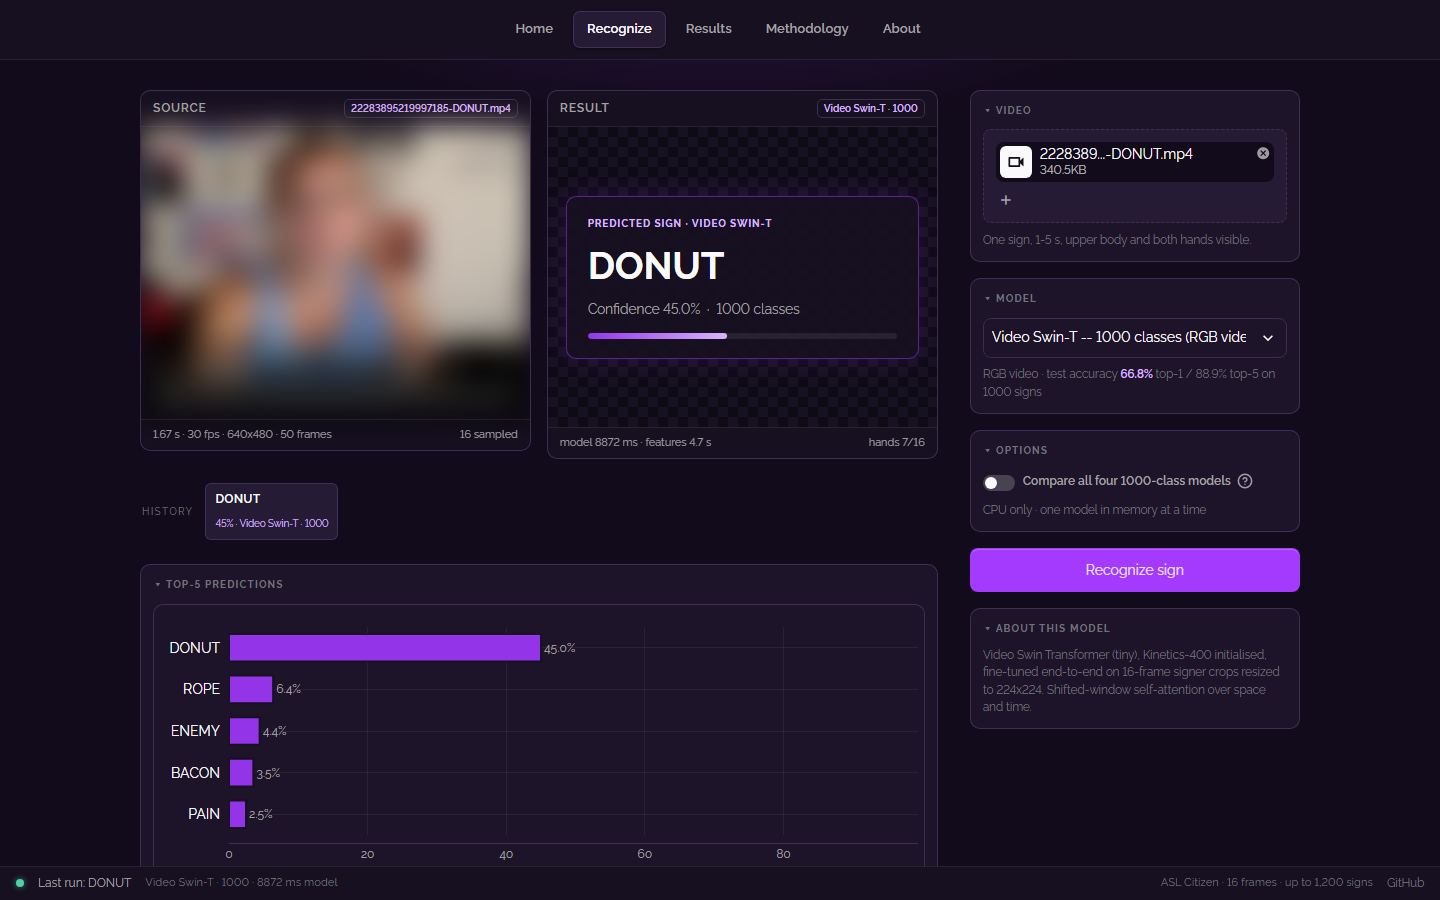
\includegraphics[width=0.92\linewidth]{ch1/app06_recognize_result.png}
\caption{The \capC{} web application recognising the sign
\gloss{DONUT} with the \swin{} model. It shows the predicted gloss, its
confidence and the five most likely signs. The uploaded video is blurred
here to protect the signer's identity.}
\label{fig:app-preview}
\end{figure}

% ---------------------------------------------------------------------
\section{Problem Statement and Analysis}
\label{sec:problem}
% ---------------------------------------------------------------------

\subsection{Problem statement}

People who use American Sign Language still have no reliable, widely
available way to communicate with non-signers when no interpreter is
present. Automatic sign language recognition could help to close this
gap, but current word-level recognition systems are not yet ready for
everyday use. Most are trained and tested on vocabularies of only a few
hundred signs, far fewer than everyday conversation needs. Many are
evaluated on the same people they were trained on, so their accuracy on
new users is unknown. The most accurate systems rely on large video models
that need a GPU, while lightweight systems that run on ordinary computers
are usually much less accurate. Finally, very few research systems ever
reach the people they are meant to serve, because they exist only as
research code. The problem addressed in this project is therefore to build
a word-level ASL recognition system that recognises an isolated sign from
an ordinary video clip, within a vocabulary of at least 1,000 signs, that
works reliably for signers it has never seen, and that runs on ordinary
CPU hardware so that it can be offered to anyone as a free web
application. Because no single architecture is known to be best on all of
these requirements at once, the problem also involves designing and
comparing several architectures to find the best balance between accuracy
and computational cost.

Formally, we treat word-level recognition as closed-vocabulary video
classification. A clip is reduced to $T=16$ frames,
$\mathbf{X} = (\mathbf{x}_1, \dots, \mathbf{x}_T)$, where each
$\mathbf{x}_t$ is an RGB frame, a vector of body landmark coordinates, or
both. Given a vocabulary $\mathcal{V} = \{1, \dots, K\}$ of glosses, the
system must learn a model $f_\theta$ that outputs a probability
distribution over $\mathcal{V}$ and predicts the most probable gloss,
\begin{equation}
  \hat{y} \;=\; \arg\max_{k \in \mathcal{V}} \; p_\theta(k \mid \mathbf{X}),
  \qquad
  p_\theta(\cdot \mid \mathbf{X}) = \operatorname{softmax}\!\big(f_\theta(\mathbf{X})\big),
  \label{eq:task}
\end{equation}
with $K \geq 1{,}000$, evaluated only on signers who do not appear in the
training data.

\subsection{Analysis of the problem}

Recognising signs from video is harder than it may first appear. An
analysis of the task and of the literature reviewed in \cref{ch:related}
shows five main challenges, which any practical solution must address.

\begin{enumerate}[label=\textbf{C\arabic*.}, leftmargin=2.6em]
  \item \textbf{Large vocabularies of similar-looking signs.} Many signs
  differ only slightly in handshape, movement or location, and some
  related words (for example \gloss{BATHROOM} and \gloss{TOILET}) look
  almost identical in a short clip. The more signs a system must know, the
  more such near-identical pairs it must separate. Accuracy therefore
  drops as the vocabulary grows. On WLASL, for example, the published I3D
  baseline falls from 65.9\,\% \topone{} accuracy on 100 words to
  32.5\,\% on 2,000 words \cite{li2020wlasl}.

  \item \textbf{Variation between signers.} People differ in body size,
  signing speed, handedness and style, and they record themselves with
  different cameras, lighting and backgrounds. A system that performs well
  on the people it was trained on can fail on new users. On the Turkish
  AUTSL dataset, for instance, accuracy fell to about 62\,\% for signers
  not seen during training \cite{sincan2020autsl}. A useful system must
  be trained and evaluated on separate groups of signers.

  \item \textbf{Few training examples per sign.} Recording and labelling
  sign videos is slow and expensive, so datasets contain few examples of
  each sign: about 10 per word in WLASL \cite{li2020wlasl} and about 31
  in \aslc{} \cite{desai2023aslcitizen}, of which roughly half are
  available for training. Large models trained on so little data tend to
  memorise the training clips instead of learning the sign.

  \item \textbf{Information spread over space and time.} The meaning of a
  sign comes from both hands, the face and the body together, and it
  unfolds over time. A model must capture fine hand shapes as well as
  motion across the clip. RGB video carries the full visual detail but is
  expensive to process and sensitive to background and lighting.
  Landmarks extracted by tools such as \mediapipe{} are compact and
  largely unaffected by background, but they lose visual detail and fail
  when hands are blurred or overlap.

  \item \textbf{Accuracy versus cost in deployment.} A recognition system
  is only useful if people can run it. Video models that need a GPU are
  costly to host, while compact models run fast on any computer but may
  be less accurate. In addition, a deployed system must prepare a user's
  video in exactly the same way as the training data. Otherwise, its real
  accuracy can fall below its reported test accuracy without any visible
  error.
\end{enumerate}

\Cref{tab:challenges-responses} summarises how the system developed in
this project addresses each challenge. The details are given in
\cref{ch:method,ch:results}.

\begin{table}[htbp]
\centering
\caption{Challenges of word-level sign language recognition and how this
project addresses them.}
\label{tab:challenges-responses}
\small
\begin{tabularx}{\linewidth}{@{}c L{4.3cm} Y@{}}
\toprule
\rowcolor{tablehead}
\textbf{\#} & \textbf{Challenge} & \textbf{How this project addresses it} \\
\midrule
C1 & Large vocabularies of similar-looking signs
   & All models are trained and tested on 1,000 signs, and the
     vocabulary is scaled from 300 to 1,200 signs to measure its effect.
     Confusable sign pairs are analysed. \\
C2 & Variation between signers
   & Training and evaluation use the official signer-independent splits of
     \aslc{}, recorded by many people on ordinary webcams. \\
C3 & Few training examples per sign
   & Compact landmark models (1.4--1.9\,M parameters) and a video
     Transformer pretrained on a large action dataset, with strong
     regularisation. \\
C4 & Information spread over space and time
   & Four architectures that model the problem differently are compared:
     RGB video, landmarks as a sequence, landmarks as a graph, and RGB
     combined with landmarks. \\
C5 & Accuracy versus cost in deployment
   & Model size and CPU latency are measured for every model. A free,
     CPU-only web application reproduces the training preprocessing and is
     verified against it. \\
\bottomrule
\end{tabularx}
\end{table}

% ---------------------------------------------------------------------
\section{Project Objectives}
\label{sec:objectives}
% ---------------------------------------------------------------------

The overall aim of the project is to design, evaluate and deploy a
word-level ASL recognition system that generalises to unseen signers on a
vocabulary of at least 1,000 signs and runs on ordinary hardware. The
specific objectives are:

\begin{enumerate}[label=\textbf{O\arabic*.}, leftmargin=2.6em]
  \item To survey deep-learning approaches to sign language recognition and
  identify the research gaps that should guide the design
  (\capA{}).
  \item To build a dual-stream appearance-plus-landmark recognition model
  and test how its accuracy changes with vocabulary size while the amount
  of data per class is held fixed (\capB{}).
  \item To find out why the dual-stream model was limited, and to design
  better architectures: a geometry-only Transformer, a skeleton graph
  network (ST-GCN) and a video Transformer (\swin{}).
  \item To compare all architectures fairly on the same 1,000 signs and
  the same signer-independent split, using \topone{}, \topfive{}, macro
  precision, recall and F1, model size, and CPU latency.
  \item To build and deploy a free web application that lets any user
  upload a sign video and receive a prediction from any trained model,
  with preprocessing that matches training, and to test its correctness,
  speed and memory use.
\end{enumerate}

% ---------------------------------------------------------------------
\section{Project Contributions}
\label{sec:contributions}
% ---------------------------------------------------------------------

The main contributions of this work are as follows.

\begin{enumerate}[leftmargin=2em]
  \item \textbf{A documented development history.} We record the full path
  from a landmark-only LSTM concept, through successive refinements of the
  dual-stream model and a move from WLASL to \aslc{}, to the final models. The
  record includes the bugs, dead ends and negative results along the way.
  In particular, it shows that the limit on our WLASL results was data
  per class, not model capacity.

  \item \textbf{A controlled vocabulary-scaling study.} We trained models
  at 300, 500, 1,000 and 1,200 signs with the median number of videos per
  class fixed at about 31. Any change in accuracy can therefore be
  attributed to vocabulary size, not to having less data per class. The
  study also showed that test-time augmentation \emph{reduces} accuracy at
  every vocabulary size we tested.

  \item \textbf{A stream ablation that identifies the bottleneck.}
  Removing the 3D-CNN appearance stream, while keeping the landmark input
  and training recipe largely unchanged, raised 1,000-sign test
  \topone{} accuracy from 28.2\,\% to 57.5\,\%. Across vocabulary sizes,
  the geometry-only model reaches 63.2\,\% (300 signs) to 57.5\,\%
  (1,000 signs).

  \item \textbf{A fair multi-architecture comparison at 1,000 signs.}
  Four architectures are compared on one class list and one
  signer-independent split of 12,560 test clips (\cref{tab:headline}).
  \swin{} is the most accurate model, with 66.8\,\% \topone{} and
  88.9\,\% \topfive{}. The \geotr{} reaches 57.5\,\% with 15 times
  fewer parameters and runs about 400 times faster on a CPU (3~ms against
  1,220~ms). Validation \topone{} accuracy also exceeds the 70\,\% gate
  set in \capA{} for the first time (74.6\,\% for \swin{}).

  \item \textbf{A deployed, tested application.} A Streamlit web
  application \cite{streamlit2026} serves all seven trained models on
  free CPU hosting. Model weights are downloaded on demand from Hugging
  Face \cite{huggingface2026hub}, and only one model is kept in memory at
  a time, with peak memory of about 830~MB. A parity test on 30 unseen
  test videos shows that the application's predictions match predictions
  on the training features for 83--87\,\% of clips with the two best
  models. Repeated runs on the same video give identical predictions.
  The application is publicly available at \AppURL{}, and its source code
  at \RepoURL{}.
\end{enumerate}

\begin{table}[htbp]
\centering
\caption{Headline results on the 1,000-sign \aslc{} test split (12,560
clips, signers unseen in training). The \rthreed{} model is the final
\capB{} model; the other three were developed after \capB{}. Latency is the CPU time of
the model forward pass only, measured on a 2-thread Kaggle CPU.}
\label{tab:headline}
\small
\setlength{\tabcolsep}{4pt}
\begin{tabular}{@{}l l c c r r@{}}
\toprule
\rowcolor{tablehead}
\textbf{Model} & \textbf{Input} & \textbf{Top-1} &
\textbf{Top-5} & \textbf{Params} & \textbf{Latency} \\
\midrule
\rthreed{}   & RGB + landmarks & 28.2\,\% & 55.1\,\% & 35.3\,M & 457~ms \\
\stgcn{}     & Landmarks       & 48.8\,\% & 74.0\,\% & 1.37\,M & 10~ms \\
\geotr{}     & Landmarks       & 57.5\,\% & 81.8\,\% & 1.91\,M & 3~ms \\
\swin{}      & RGB video       & \textbf{66.8\,\%} & \textbf{88.9\,\%} & 28.6\,M & 1,220~ms \\
\bottomrule
\end{tabular}
\end{table}

% ---------------------------------------------------------------------
\section{Project Outlines}
\label{sec:outline}
% ---------------------------------------------------------------------

The rest of this report is organised as follows.

\begin{description}[leftmargin=0pt, labelsep=0.5em, font=\normalfont\bfseries]
  \item[\Cref{ch:related}: Related Works] reviews the literature surveyed in
  \capA{} in three groups. These are CNN--recurrent and landmark-based
  approaches; Transformer, graph-based and multi-stream fusion
  architectures; and datasets, low-resource sign languages and
  self-supervised learning. The chapter ends with a summary table and the
  research gap.

  \item[\Cref{ch:method}: Materials and Method] describes the dataset, the
  preprocessing and feature-extraction pipeline, and the four
  architectures, with the reasons for each design decision. It covers the
  development path from \capB{} to the post-\capB{} redesign, the training
  setup and evaluation metrics, and the design of the web application and
  how the models are integrated into it.

  \item[\Cref{ch:data}: Data Description] describes \aslc{} and the
  vocabulary subsets used in this work, their characteristics and the data
  analysis plan.

  \item[\Cref{ch:results}: Results and Discussion] reports the results of
  all trained models. It analyses vocabulary scaling, per-class errors and
  confusable sign pairs, the accuracy--latency trade-off, and the
  application's parity, latency and memory tests.

  \item[\Cref{ch:conclusion}: Conclusion] summarises the overall
  contribution, states the limitations of the work, and outlines future
  directions, including continuous (sentence-level) recognition.
\end{description}

\noindent The bibliography is followed by \cref{app:a}, which contains
additional figures and implementation details, and by the mapping of the
project to the course and program outcomes of CSE400 A, B and C.
